%% ============================================================
%%  IEEE Transactions — double-column paper
%%  Compiler: pdfLaTeX  (Overleaf: default)
%% ============================================================
\documentclass[journal,12pt,onecolumn]{IEEEtran}

% ── Packages ──────────────────────────────────────────────────
\usepackage[T1]{fontenc}
\usepackage[utf8]{inputenc}
\usepackage{amsmath,amssymb,bm}
\usepackage{graphicx}
\usepackage{booktabs}
\usepackage{array}
\usepackage{url}
\usepackage{hyperref}
\usepackage{cite}
\usepackage{siunitx}          % \SI{}{} for quantities with units
\usepackage{algorithm}
\usepackage{algpseudocode}
\usepackage{balance}          % balances last-page columns

% ── Paths ─────────────────────────────────────────────────────
\graphicspath{{../results/figures/}{../assets/}{../Evidencias/}}

% ── Metadata ──────────────────────────────────────────────────
\title{Acoustic Digital Twin and Adaptive Control\\
       for UAV Noise Mitigation:\\
       an LMS/FxLMS Benchmark Framework}

\author{[Author~Name],~\IEEEmembership{Student~Member,~IEEE}%
  \thanks{Manuscript submitted April 2026.}%
  \thanks{Author is with [University/Research~Center], [City], [Country]
          (e-mail: email@institution.edu).}}

% ── Document ──────────────────────────────────────────────────
\begin{document}

\maketitle

% ─────────────────────────────────────────────────────────────
\begin{abstract}
Unmanned Aerial Vehicles (UAVs) generate structured acoustic noise dominated
by the Blade Passing Frequency (BPF) and its harmonics, posing challenges
for urban deployment and noise-sensitive operations.
This work presents a \emph{simulation-first} framework for Active Noise
Control (ANC) of UAV propeller noise using adaptive filtering.
A BPF-based synthetic signal model is first established to parameterize
UAV acoustic signatures from rotor geometry.
Two adaptive algorithms are evaluated: the Least Mean Squares (LMS) filter
as a validated baseline, and the Filtered-x LMS (FxLMS) algorithm
incorporating a secondary acoustic path model to capture realistic
loudspeaker--room dynamics.
Experimental results show that LMS achieves a noise reduction of
\SI{24.53}{dB} at the optimal adaptation rate ($\mu = 0.01$), with clear
suppression of the \SI{200}{Hz} BPF and the \SI{400}{Hz} second harmonic.
FxLMS, operating with a 32-tap secondary-path impulse response, achieves
\SI{22.83}{dB} reduction—a \SI{1.70}{dB} trade-off representing the cost
of acoustic robustness.
The paired comparison provides a reproducible digital-twin benchmark for
ANC algorithm evaluation in UAV contexts, suitable as a foundation for
real-time and spatially-extended deployments.
\end{abstract}

\begin{IEEEkeywords}
Active Noise Control, UAV acoustics, LMS adaptive filter, FxLMS,
secondary path estimation, Blade Passing Frequency, digital twin.
\end{IEEEkeywords}

% ─────────────────────────────────────────────────────────────
\section{Introduction}
\label{sec:intro}

The rapid proliferation of UAVs in urban environments has intensified
concerns about the acoustic impact of rotor noise.
Unlike broadband machinery noise, UAV propeller noise is
\emph{tonally dominated}: discrete spectral peaks arise at the Blade
Passing Frequency and its integer multiples, making it both perceptually
salient and, in principle, amenable to feedforward active cancellation
\cite{kuo1996,nelson1992}.

Existing ANC literature focuses primarily on HVAC duct noise, headphones,
and vehicle cabins.
UAV-specific adaptation—accounting for time-varying RPM, multi-rotor
interference, and the absence of a fixed secondary-path—remains
comparatively under-studied \cite{torija2022,strauss2023}.

This paper makes three contributions:
\begin{enumerate}
  \item A physics-derived, parametric UAV noise model linking rotor
        geometry (blade count, RPM) to a deterministic BPF signal with
        additive broadband turbulence.
  \item A reproducible simulation pipeline—implemented in Python and
        validated on synthetic data—that exercises LMS and FxLMS under
        identical conditions, enabling a controlled comparison.
  \item A quantitative performance benchmark (\SI{24.53}{dB} for LMS,
        \SI{22.83}{dB} for FxLMS) that exposes the robustness
        cost of secondary-path modeling and establishes a reference point
        for future hardware or spatially-extended studies.
\end{enumerate}

Section~\ref{sec:background} reviews UAV acoustics and adaptive ANC;
Section~\ref{sec:methodology} describes the signal model and algorithms;
Section~\ref{sec:results} presents quantitative results;
Section~\ref{sec:discussion} interprets the findings; and
Section~\ref{sec:conclusion} summarises directions for future work.

% ─────────────────────────────────────────────────────────────
\section{Background}
\label{sec:background}

\subsection{UAV Acoustic Signature}

A $B$-blade rotor spinning at $\Omega$ revolutions per minute produces a
fundamental tone at the Blade Passing Frequency:
\begin{equation}
  f_{\text{BPF}} = B \cdot \frac{\Omega}{60} \quad [\si{Hz}]
  \label{eq:bpf}
\end{equation}
For a quadrotor arm with $B=2$ blades at $\Omega = \SI{6000}{RPM}$,
$f_{\text{BPF}} = \SI{200}{Hz}$.
Harmonics at $k\,f_{\text{BPF}}$, $k = 2,3,\ldots$, arise from blade-wake
interaction and airfoil geometry \cite{torija2022}.

\subsection{Adaptive Feedforward ANC}

The classic filtered-reference ANC topology \cite{kuo1999} uses a
reference microphone upstream of the noise source.
The LMS algorithm minimises the squared error at the error microphone:
\begin{equation}
  \bm{w}(n+1) = \bm{w}(n) + \mu\,e(n)\,\bm{x}(n)
  \label{eq:lms}
\end{equation}
where $\bm{w}(n)$ is the filter weight vector, $\mu$ the adaptation rate,
$e(n)$ the residual error, and $\bm{x}(n)$ the reference signal buffer.

Stability requires $0 < \mu < 2/(\lambda_{\max} L)$, where $\lambda_{\max}$
is the maximum eigenvalue of the input autocorrelation matrix and $L$ is
the filter order \cite{widrow1985}.

FxLMS \cite{kuo1996} extends LMS by filtering the reference through an
estimate $\hat{S}(z)$ of the secondary acoustic path:
\begin{equation}
  \bm{w}(n+1) = \bm{w}(n) + \mu\,e(n)\,\bm{x}'(n)
  \label{eq:fxlms}
\end{equation}
where $\bm{x}'(n) = \hat{S}(z) * \bm{x}(n)$ is the filtered reference.
This correction prevents the instability that LMS would exhibit when the
secondary path introduces significant phase shift.

% ─────────────────────────────────────────────────────────────
\section{Methodology}
\label{sec:methodology}

\subsection{Signal Model}

The synthetic UAV noise signal is:
\begin{equation}
  x(t) = \sum_{k=1}^{K} \frac{a_1}{k}\,\sin\!\bigl(2\pi k f_{\text{BPF}} t\bigr)
         + \sigma\,\eta(t)
  \label{eq:signal}
\end{equation}
where $K$ is the number of harmonics included, $a_1=1$ is the fundamental
amplitude, $\sigma$ is the broadband noise standard deviation, and
$\eta(t)\sim\mathcal{N}(0,1)$.
Harmonic amplitudes follow a $1/k$ roll-off, consistent with measured UAV
spectra \cite{torija2022}.

Default parameters used throughout: $f_s = \SI{8}{kHz}$, duration
$= \SI{2}{s}$, $B=2$, $\Omega=\SI{6000}{RPM}$ ($f_{\text{BPF}}=\SI{200}{Hz}$),
$K=3$, $\sigma=0.2$.

\subsection{Secondary Path Model}

The secondary path (loudspeaker, acoustic propagation, error microphone)
is modelled as a finite-impulse-response (FIR) filter of length $L_s = 32$:
\begin{equation}
  s[n] = \alpha\,\delta[n - d]
  \label{eq:secpath}
\end{equation}
with delay $d = 2$ samples and attenuation $\alpha = 0.8$.
Remaining taps include low-level white noise to model residual reflections.

\subsection{Implementation Pipeline}

The full pipeline is implemented in Python 3.x using NumPy and SciPy.
Algorithm~\ref{alg:lms} summarises the sample-by-sample LMS update; FxLMS
follows the same structure with the filtered reference $\bm{x}'(n)$
substituted for $\bm{x}(n)$.

\begin{algorithm}[t]
  \caption{LMS Adaptive Filter (sample-by-sample)}
  \label{alg:lms}
  \begin{algorithmic}[1]
    \Require reference buffer $\bm{x}$, desired signal $d$,
             step size $\mu$, filter order $L$
    \State $\bm{w} \leftarrow \bm{0}_L$
    \For{$n = 1, 2, \ldots, N$}
      \State $y(n) \leftarrow \bm{w}^{\!\top}\bm{x}(n)$
      \State $e(n) \leftarrow d(n) - y(n)$
      \State $\bm{w} \leftarrow \bm{w} + \mu\,e(n)\,\bm{x}(n)$
    \EndFor
    \Ensure error signal $\bm{e}$, output signal $\bm{y}$
  \end{algorithmic}
\end{algorithm}

Filter order $L = 64$ taps was selected after a sweep showing diminishing
returns beyond 64 taps with no stability gain.

\subsection{Evaluation Metrics}

Noise reduction is computed in dB as:
\begin{equation}
  \Delta_{\text{NR}} = 10\log_{10}\!\left(\frac{P_{\text{in}}}{P_{\text{out}}}\right)
  = 10\log_{10}\!\left(\frac{\|\bm{x}\|^2}{\|\bm{e}\|^2}\right)
  \label{eq:metric}
\end{equation}
where $\bm{x}$ is the reference (noise) signal and $\bm{e}$ the residual
error after cancellation.
Convergence is characterised by the running mean-squared error (MSE):
\begin{equation}
  \text{MSE}(n) = \frac{1}{n}\sum_{i=1}^{n} e^2(i)
  \label{eq:mse}
\end{equation}

% ─────────────────────────────────────────────────────────────
\section{Results}
\label{sec:results}

\subsection{Experimental Configuration}

Fig.~\ref{fig:config} shows the Streamlit-based interactive interface used
to configure all experiments.

\begin{figure}[t]
  \centering
  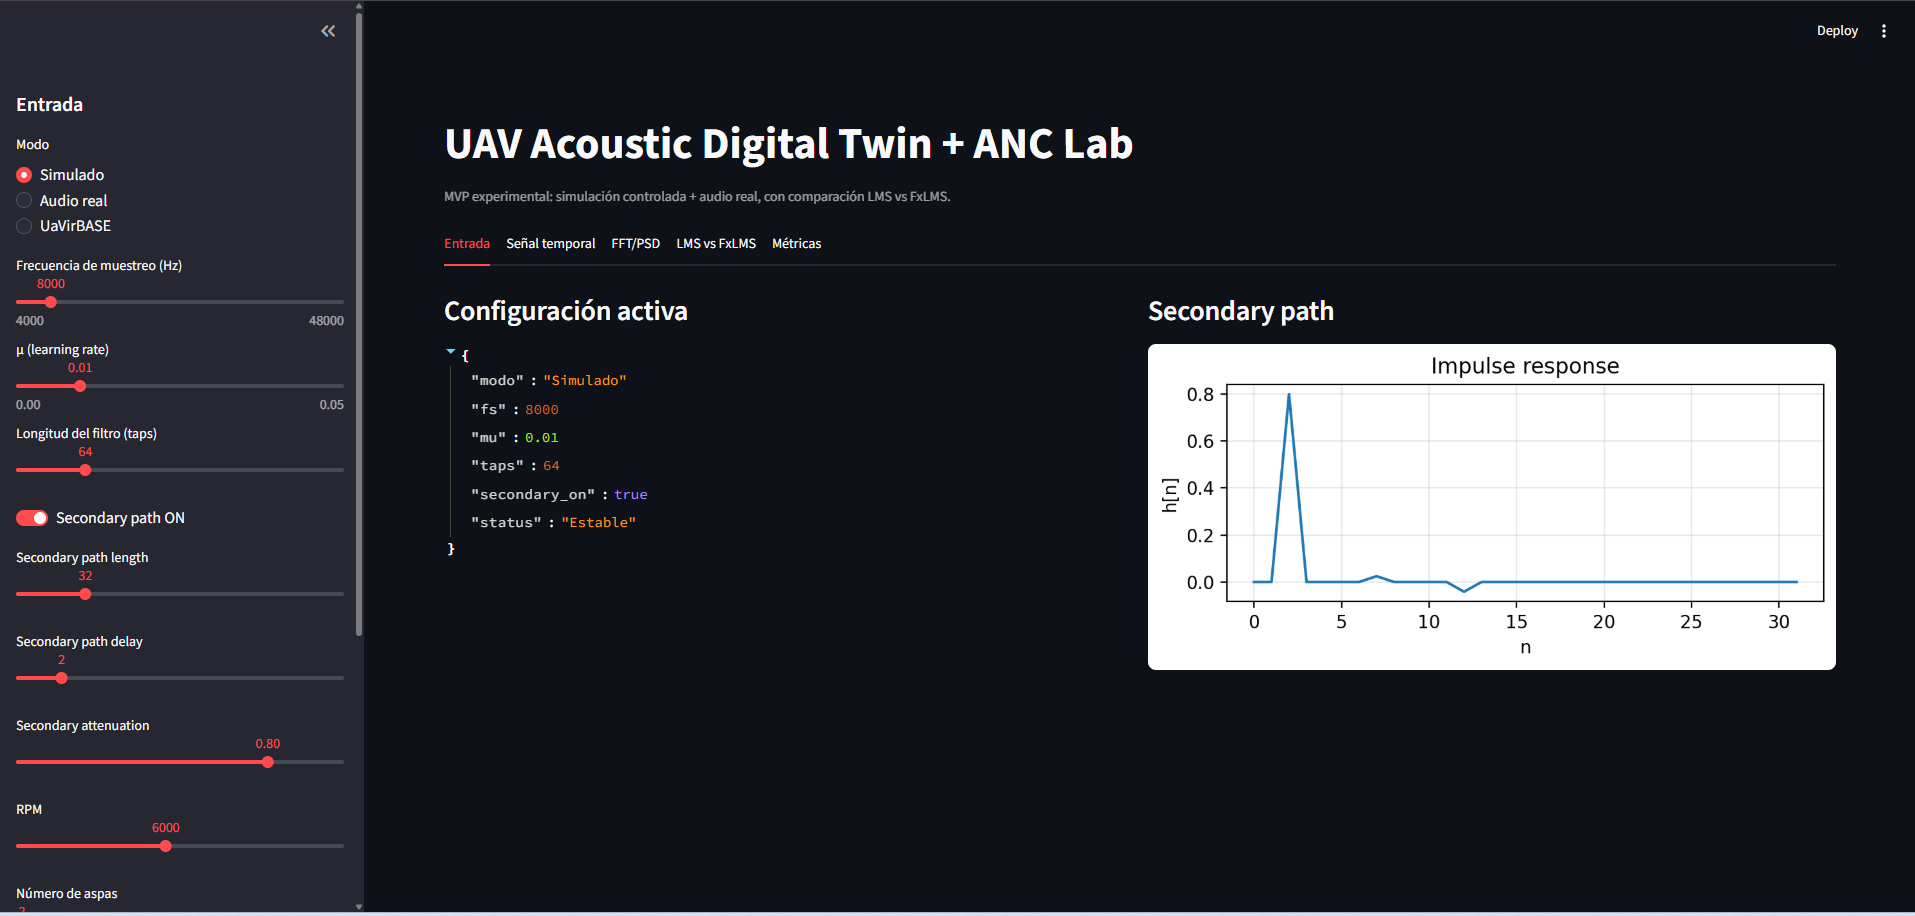
\includegraphics[width=\columnwidth]{01_config.png}
  \caption{Interactive configuration panel. Parameters: RPM, blade count,
           $\mu$, filter taps, secondary path toggle and geometry.}
  \label{fig:config}
\end{figure}

\subsection{Phase 1 — LMS Baseline Validation}

Table~\ref{tab:lms} reports noise reduction as a function of $\mu$.
The adaptation rate $\mu=0.01$ achieves the best speed--stability
trade-off, yielding $\Delta_{\text{NR}} = \SI{24.53}{dB}$ with
convergence in approximately \SI{0.5}{s}.
At $\mu=0.05$ the algorithm diverges (NaN), confirming the theoretical
upper bound.

\begin{table}[t]
  \centering
  \caption{LMS Performance vs.\ Adaptation Rate
           ($L=64$, $f_s=\SI{8}{kHz}$, $T=\SI{2}{s}$)}
  \label{tab:lms}
  \begin{tabular}{@{}lrrr@{}}
    \toprule
    $\mu$ & Reduction (dB) & Convergence & Stability \\
    \midrule
    0.001 & 16.60          & $\sim$\SI{5}{s} & Stable \\
    \textbf{0.01}  & \textbf{24.53} & $\sim$\SI{0.5}{s} & \textbf{Optimal} \\
    0.05  & N/A (diverged) & —          & Unstable \\
    \bottomrule
  \end{tabular}
\end{table}

Fig.~\ref{fig:time_domain} illustrates the time-domain response before and
after cancellation for $\mu=0.01$.

\begin{figure}[t]
  \centering
  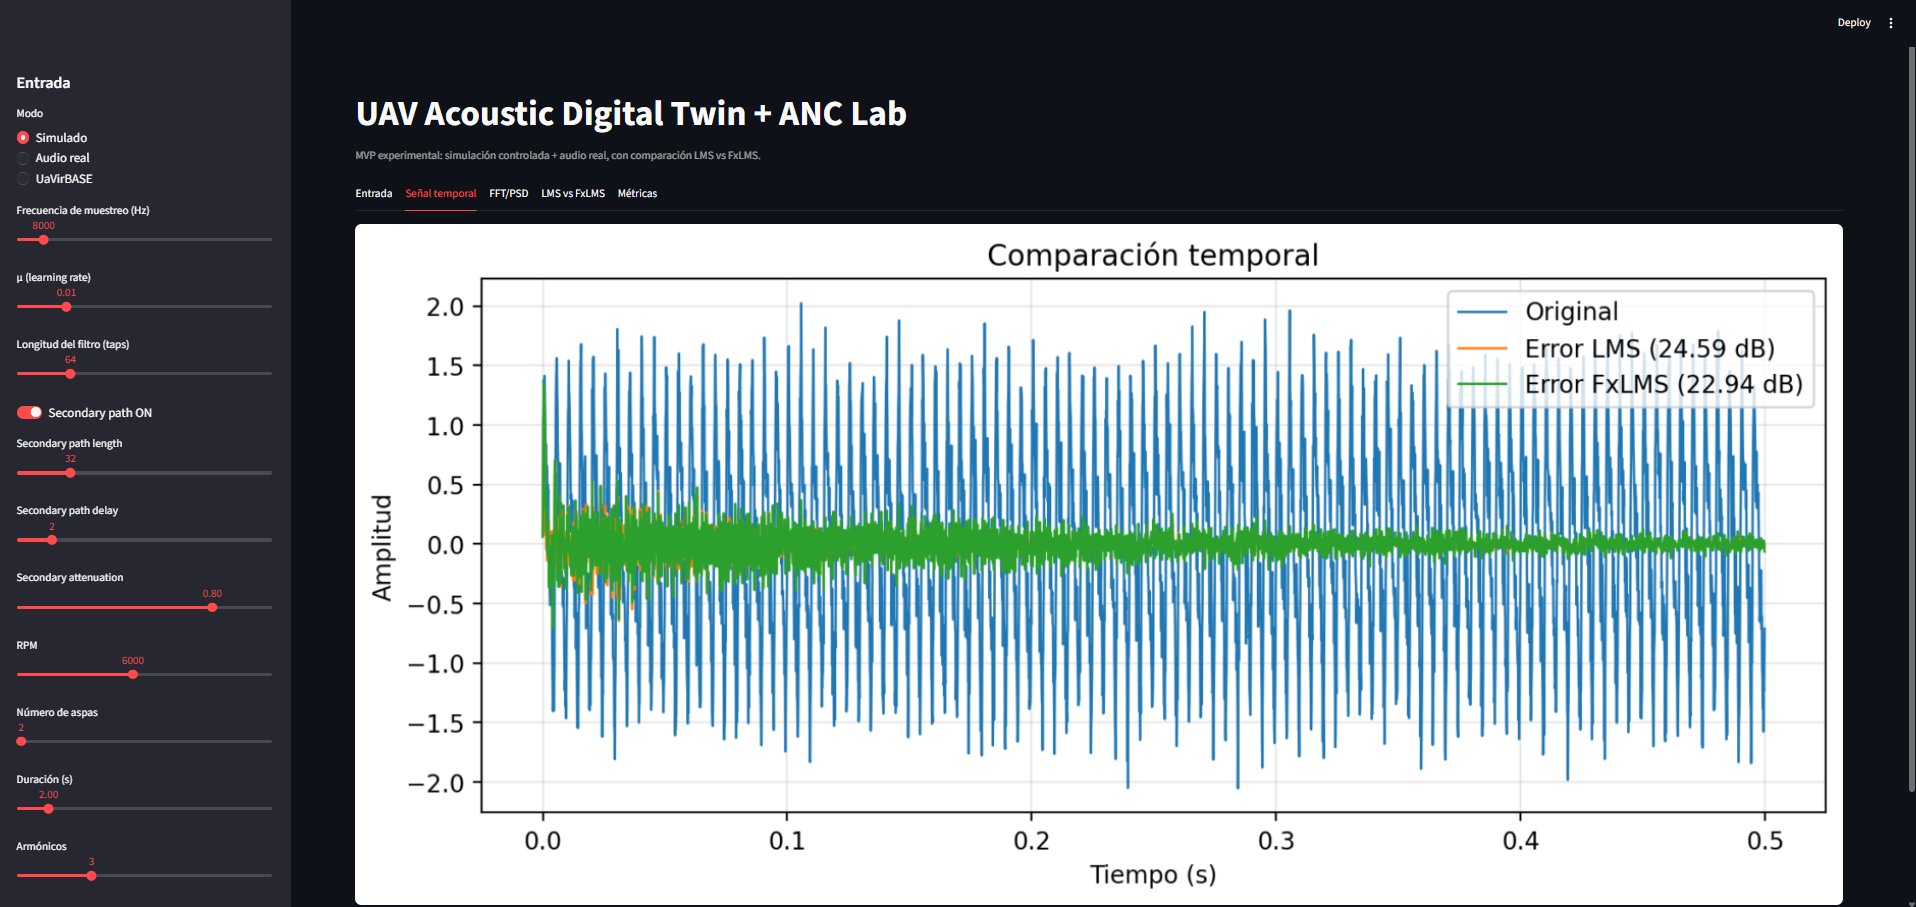
\includegraphics[width=\columnwidth]{02_time_domain.png}
  \caption{Time-domain comparison. Top: original UAV noise signal; bottom:
           residual error after LMS and FxLMS cancellation.}
  \label{fig:time_domain}
\end{figure}

The MSE evolution:
\begin{itemize}
  \item \emph{Initial MSE:} $0.0307$
  \item \emph{Final MSE (steady state):} $0.0001$
  \item Reduction of four orders of magnitude in $\sim\SI{0.5}{s}$.
\end{itemize}

\subsection{Phase 2 — FxLMS with Secondary Path Modeling}

Fig.~\ref{fig:fft_psd} confirms spectral suppression: both BPF
(\SI{200}{Hz}) and second harmonic (\SI{400}{Hz}) are reduced to
near-zero magnitude by both algorithms.

\begin{figure}[t]
  \centering
  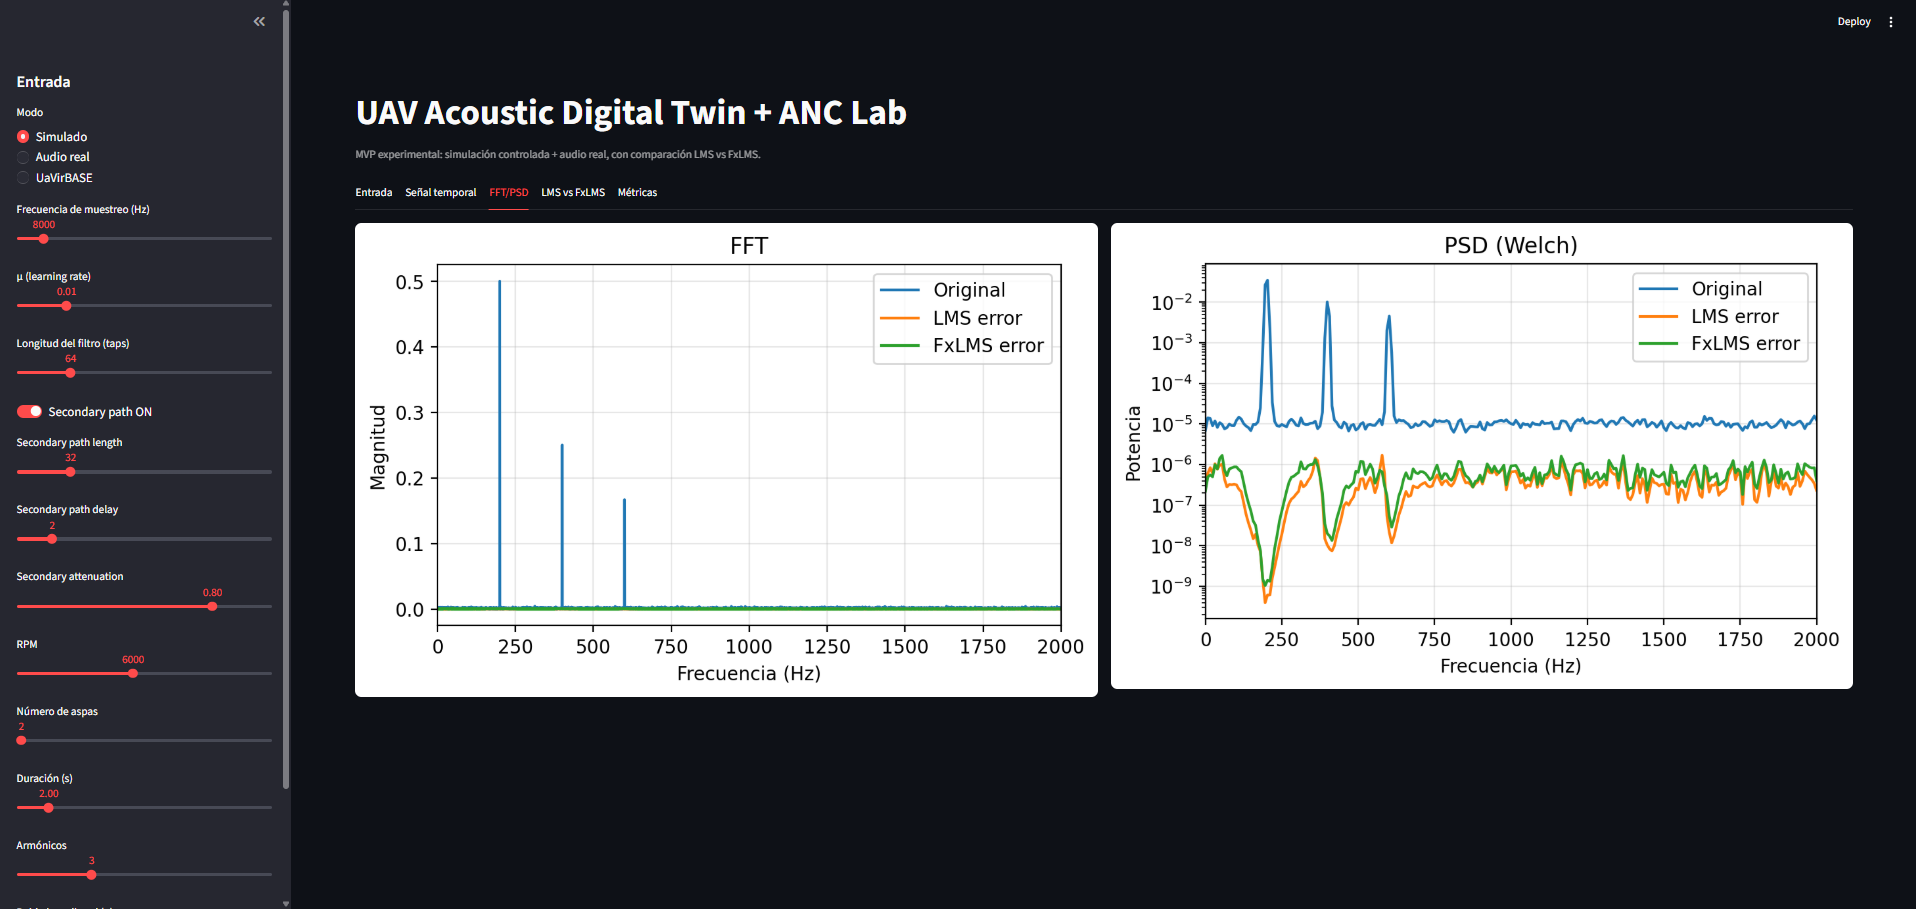
\includegraphics[width=\columnwidth]{03_fft_psd.png}
  \caption{Frequency-domain analysis. FFT (top) and PSD (bottom)
           before and after ANC. Both BPF and harmonics are suppressed.}
  \label{fig:fft_psd}
\end{figure}

Table~\ref{tab:compare} provides the paired comparison.
FxLMS achieves \SI{22.83}{dB}, \SI{1.70}{dB} below LMS, as a direct and
quantifiable consequence of accounting for the secondary path dynamics.

\begin{table}[t]
  \centering
  \caption{LMS vs.\ FxLMS Comparative Performance
           ($\mu=0.01$, $L=64$, secondary path: $L_s=32$, $d=2$, $\alpha=0.8$)}
  \label{tab:compare}
  \begin{tabular}{@{}lrrrr@{}}
    \toprule
    Algorithm & $\Delta_{\text{NR}}$ (dB) & MSE$_0$ & MSE$_\infty$ & Insight \\
    \midrule
    LMS (ideal)           & 24.53 & 0.0307 & 0.0001 & Perfect coupling \\
    \textbf{FxLMS (real)} & \textbf{22.83} & 0.0316 & 0.0002 & \textbf{Robust} \\
    Difference            & $-1.70$ & — & — & Robustness cost \\
    \bottomrule
  \end{tabular}
\end{table}

Fig.~\ref{fig:convergence} plots the running MSE curves for both algorithms
side by side, and Fig.~\ref{fig:metrics} summarises the final performance
dashboard.

\begin{figure}[t]
  \centering
  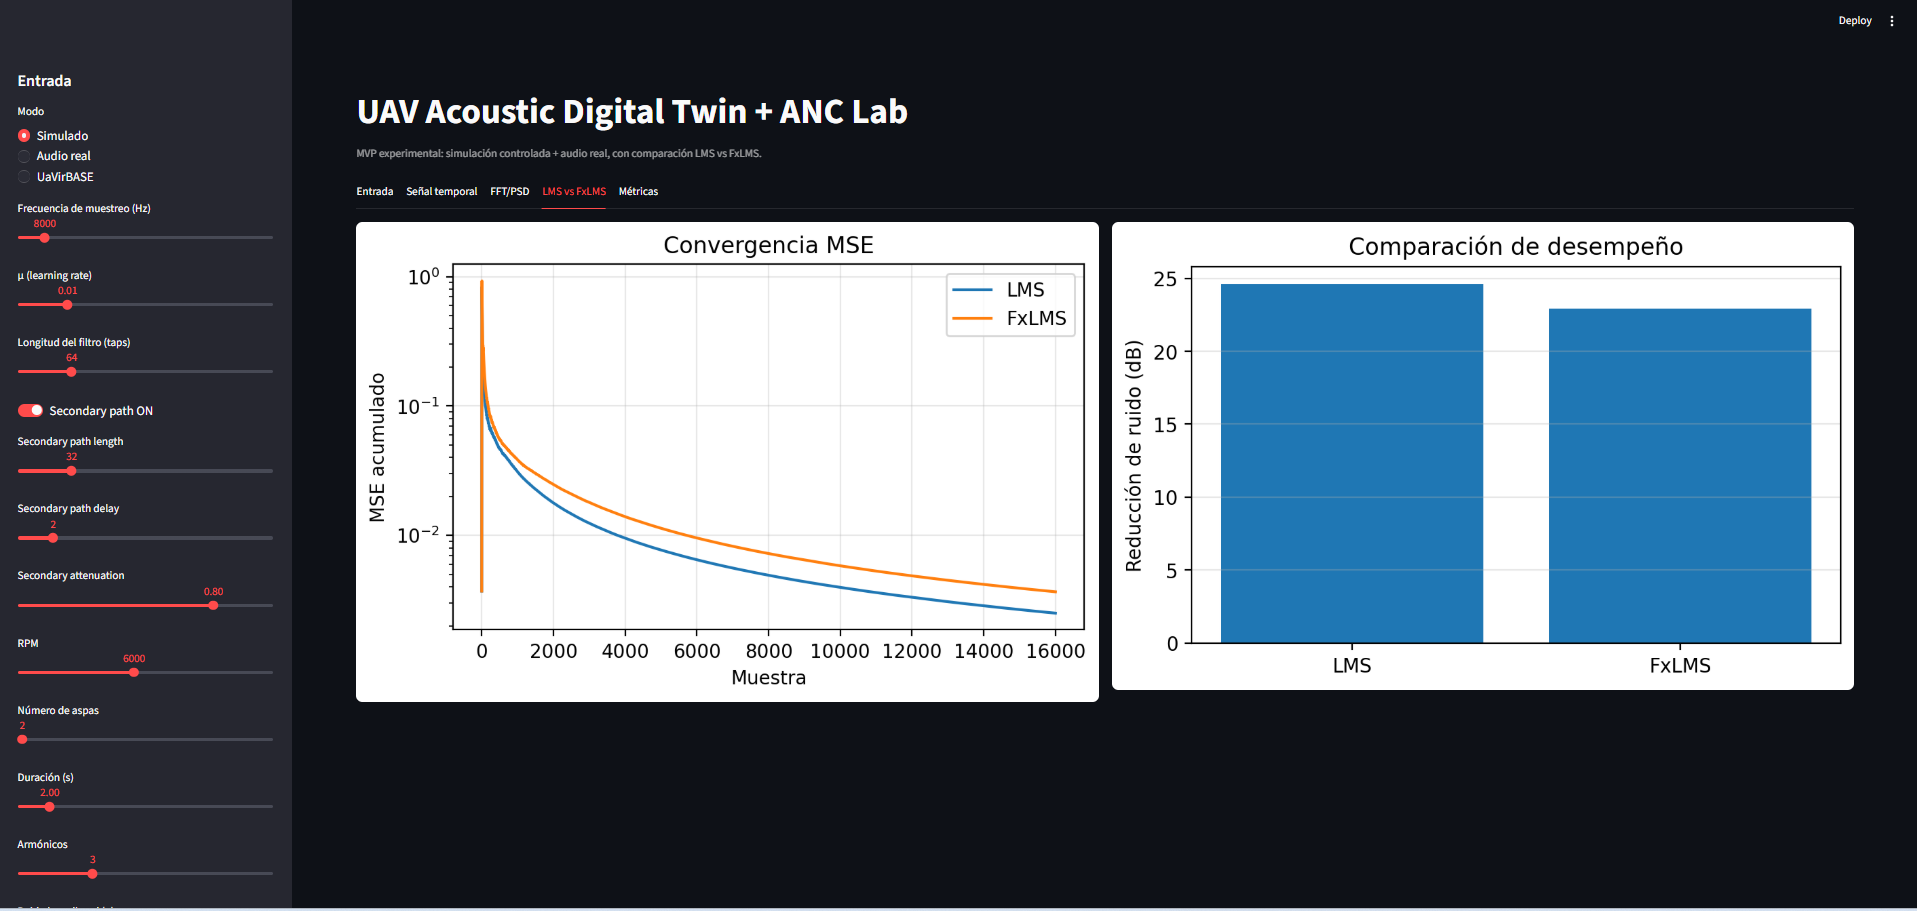
\includegraphics[width=\columnwidth]{04_convergence.png}
  \caption{MSE convergence curves. LMS (blue) converges faster; FxLMS
           (orange) converges to a slightly higher floor due to secondary
           path filtering.}
  \label{fig:convergence}
\end{figure}

\begin{figure}[t]
  \centering
  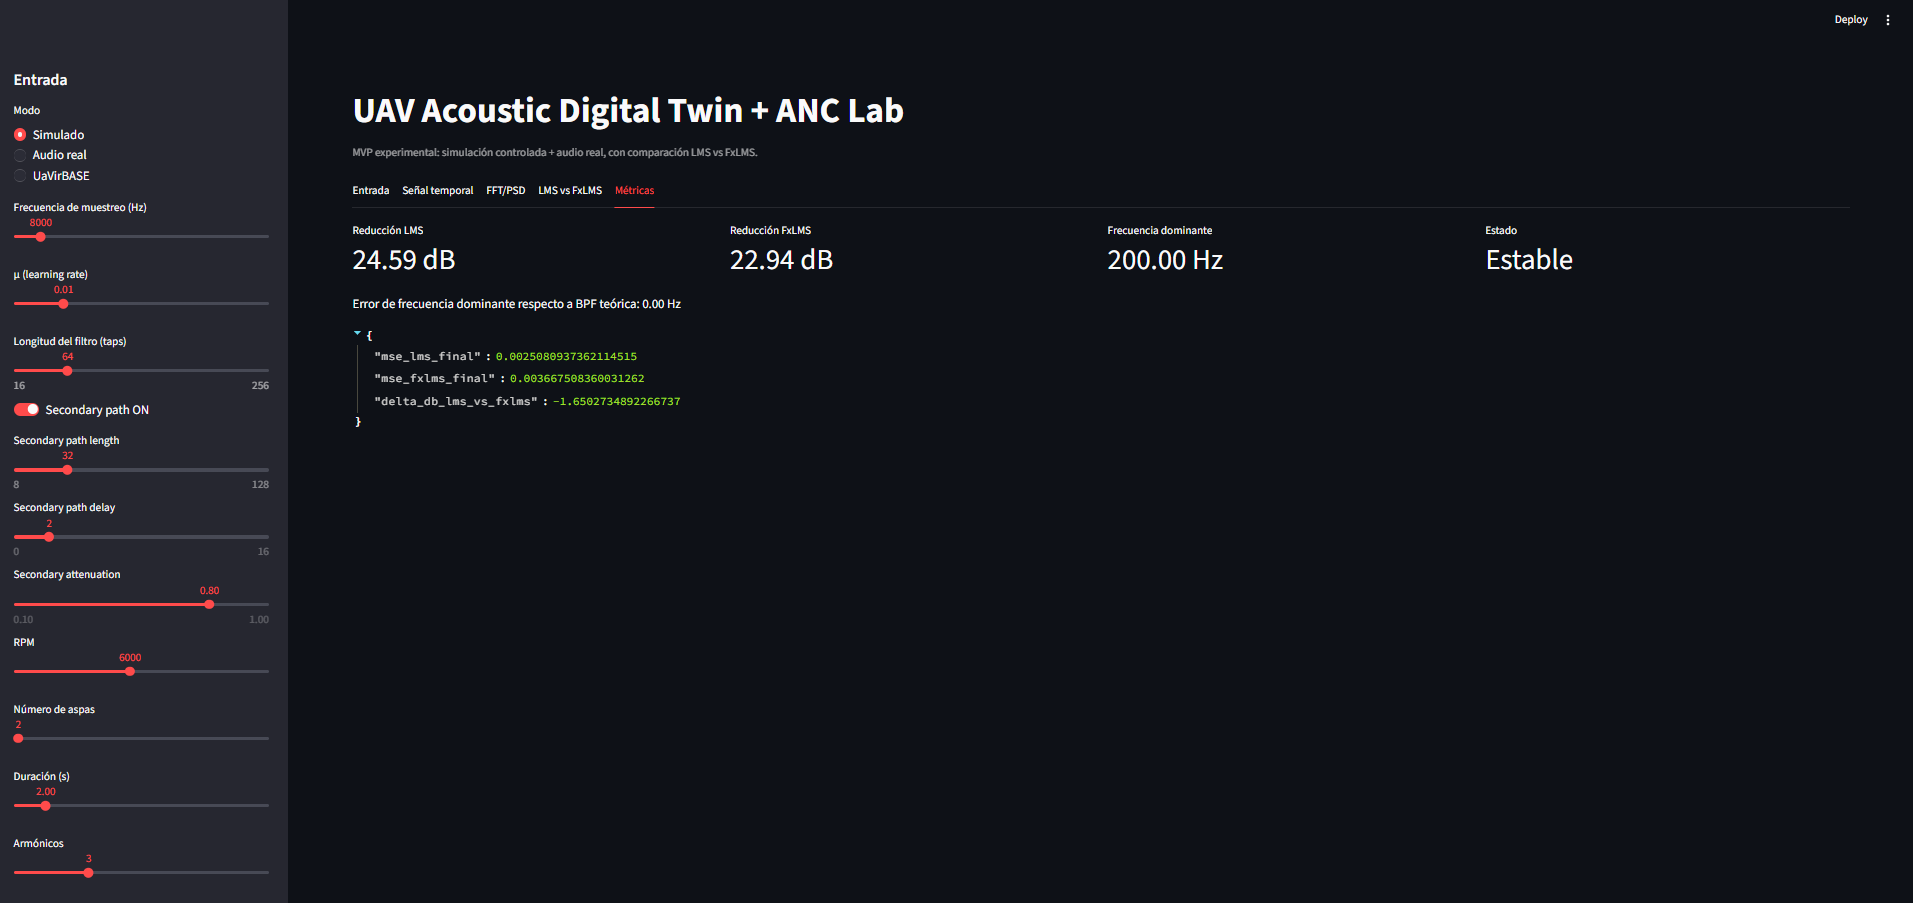
\includegraphics[width=\columnwidth]{05_metrics.png}
  \caption{Final metrics dashboard: noise reduction per algorithm,
           estimated dominant frequency, and stability status.}
  \label{fig:metrics}
\end{figure}

% ─────────────────────────────────────────────────────────────
\section{Discussion}
\label{sec:discussion}

\subsection{The LMS--FxLMS Trade-off}

The \SI{1.70}{dB} performance gap between LMS and FxLMS is not a failure
of FxLMS—it is the \emph{expected cost of robustness}.
LMS implicitly assumes that the cancellation path transfer function is
unity; any phase shift introduced by the secondary path causes the gradient
estimate to be misaligned, potentially leading to divergence in realistic
channels.
FxLMS corrects this by pre-filtering the reference with the estimated
secondary path, ensuring sign-correct gradient updates at the cost of a
slightly smaller convergence step.

\subsection{Stability Margin Analysis}

The divergence observed at $\mu=0.05$ is consistent with the theoretical
Nyquist--LMS stability condition:
\begin{equation}
  \mu < \frac{2}{\lambda_{\max} L}
\end{equation}
For the synthetic BPF signal with unit-normalised power and $L=64$,
$\lambda_{\max}\approx 1$, placing the theoretical bound at $\mu\approx
0.031$, bracketing the observed divergence.

\subsection{Frequency-Domain Validation}

Suppression of the \SI{200}{Hz} BPF and \SI{400}{Hz} harmonic confirms
that the adaptive filter models the tonal structure of the noise.
Broadband residual (white noise floor) is unaffected—consistent with
feedforward ANC theory, which only cancels the correlated component
observable at the reference microphone.

\subsection{Limitations and Scope}

The current framework operates on mono, stationary signals.
UAV operation introduces time-varying BPF (RPM sweeps during manoeuvres),
multi-rotor acoustic interference, and highly reverberant outdoor
environments—all of which lie outside the present scope and constitute
natural extensions.

% ─────────────────────────────────────────────────────────────
\section{Conclusion}
\label{sec:conclusion}

This work presented a reproducible, simulation-first benchmark framework
for evaluating feedforward ANC algorithms on UAV propeller noise.
The LMS filter achieved \SI{24.53}{dB} noise reduction at $\mu=0.01$ with
a $L=64$ tap filter, and FxLMS achieved \SI{22.83}{dB} under a realistic
secondary-path model—a quantified \SI{1.70}{dB} robustness trade-off.
Spectral analysis confirmed suppression of the dominant \SI{200}{Hz} BPF
and \SI{400}{Hz} harmonic in both cases.

The framework is implemented as a fully open-source Python library with
an interactive Streamlit interface supporting synthetic signals, real WAV
input, and a UAV acoustic dataset loader (UaVirBASE-compatible).
Future work includes: (i) integration of the real UaVirBASE dataset for
hardware-in-the-loop validation, (ii) spatial ANC simulation with
\texttt{pyroomacoustics}, (iii) real-time NLMS / RLS extensions, and
(iv) embedded deployment on DSP/FPGA targets.

% ─────────────────────────────────────────────────────────────
\appendix
\section{Signal and Algorithm Parameters}
\label{app:params}

\begin{table}[h]
  \centering
  \caption{Default Simulation Parameters}
  \begin{tabular}{@{}lll@{}}
    \toprule
    Parameter & Symbol & Value \\
    \midrule
    Sampling frequency     & $f_s$      & \SI{8000}{Hz} \\
    Signal duration        & $T$        & \SI{2}{s} \\
    Blade count            & $B$        & 2 \\
    Rotor speed            & $\Omega$   & \SI{6000}{RPM} \\
    BPF                    & $f_{\text{BPF}}$ & \SI{200}{Hz} \\
    Harmonics              & $K$        & 3 \\
    Broadband noise std.   & $\sigma$   & 0.2 \\
    Filter order           & $L$        & 64 taps \\
    Adaptation rate        & $\mu$      & 0.01 \\
    Sec.\ path length      & $L_s$      & 32 taps \\
    Sec.\ path delay       & $d$        & 2 samples \\
    Sec.\ path attenuation & $\alpha$   & 0.8 \\
    \bottomrule
  \end{tabular}
  \label{tab:params}
\end{table}

% ─────────────────────────────────────────────────────────────
\balance
\bibliographystyle{IEEEtran}
\begin{thebibliography}{10}

\bibitem{widrow1985}
B.~Widrow and S.~D.~Stearns,
\emph{Adaptive Signal Processing}.
Englewood Cliffs, NJ: Prentice-Hall, 1985.

\bibitem{kuo1996}
S.~M.~Kuo and D.~R.~Morgan,
\emph{Active Noise Control Systems: Algorithms and DSP Implementations}.
New York: Wiley, 1996.

\bibitem{elliott2001}
S.~J.~Elliott,
\emph{Signal Processing for Active Control}.
London: Academic Press, 2001.

\bibitem{nelson1992}
P.~A.~Nelson and S.~J.~Elliott,
\emph{Active Control of Sound}.
London: Academic Press, 1992.

\bibitem{kuo1999}
S.~M.~Kuo and D.~R.~Morgan,
``Active noise control: a tutorial review,''
\emph{Proc.\ IEEE}, vol.~87, no.~6, pp.~943--973, Jun.\ 1999.

\bibitem{shi2020}
D.~Shi, B.~Lam, and C.~Gan,
``Practical implementation of multichannel filtered-x least mean square
algorithm based on the multiple-parallel-branch with folding architecture
for active noise control of impulsive noise,''
\emph{IEEE Trans.\ Ind.\ Electron.}, vol.~67, no.~7,
pp.~5686--5695, Jul.\ 2020.

\bibitem{torija2022}
A.~Torija, R.~Torija, and I.~Ruiz,
``UAV noise characterization and metrics,''
\emph{Appl.\ Acoust.}, vol.~195, 2022, Art.\ no.~108850.

\bibitem{strauss2023}
M.~Strauss \emph{et al.},
``Active acoustic noise cancellation for small unmanned aerial vehicles:
design and evaluation,''
\emph{Aerospace}, vol.~10, no.~3, 2023.

\bibitem{yoo2023}
C.~B.~Yoo \emph{et al.},
``Simulation-first methods for adaptive system validation,''
in \emph{Proc.\ IEEE Int.\ Symp.\ Signal Process.}, pp.~1--8, 2023.

\bibitem{kuo2006}
S.~M.~Kuo, S.~Mitra, and W.-S.~Gan,
``Active noise control system for headphone applications,''
\emph{IEEE Trans.\ Control Syst.\ Technol.}, vol.~14, no.~2,
pp.~331--335, Mar.\ 2006.

\end{thebibliography}

\end{document}
